\chapter{Experimental Details}

Having discussed all of the relevant theoretical aspects of the Higgs boson and its role in the Standard Model as 
well as how we can measure it in particle colliders in theory, it is now necessary to explain how this is done in 
practice. This chapter covers all experimental tools used to do so relevant to this thesis, from the Large Hadron 
Collider (LHC) that facilitates particle collisions to the ATLAS detector that records their interaction products. 
I will start with discussions about the hardware of the LHC and ATLAS and then move on to talk about object 
reconstructions within the context of our experiment.

\section{The Large Hadron Collider}

The Large Hadron Collider (LHC) is the largest proton-proton collider in the world, located at the CERN
\footnote{"Organisation européenne pour la recherche nucléaire" or in its english translation "European 
Organization for Nuclear Research"} laboratory near Geneva, Switzerland. It is a circular collider with a circumference 
of 26.7 km and can accelerate both protons and heavy ion beams to $6.8\ TeV$, leading to center of mass energies of up 
to $13.6\ TeV$ in collisions. To facilitate these collisions, the LHC accelerates two collimated beams \footnote{The 
beams are not continuous but rather consist of individual bunches that are spaced evenly} of hadrons simultaneously and 
guides them towards each other at 4 intersection points. These points correspond to the sites of the four main detectors 
located on the LHC ring: ATLAS, CMS, LHCb and ALICE. \par

%https://www.nature.com/articles/s42254-024-00758-5
\begin{figure}
\centering
    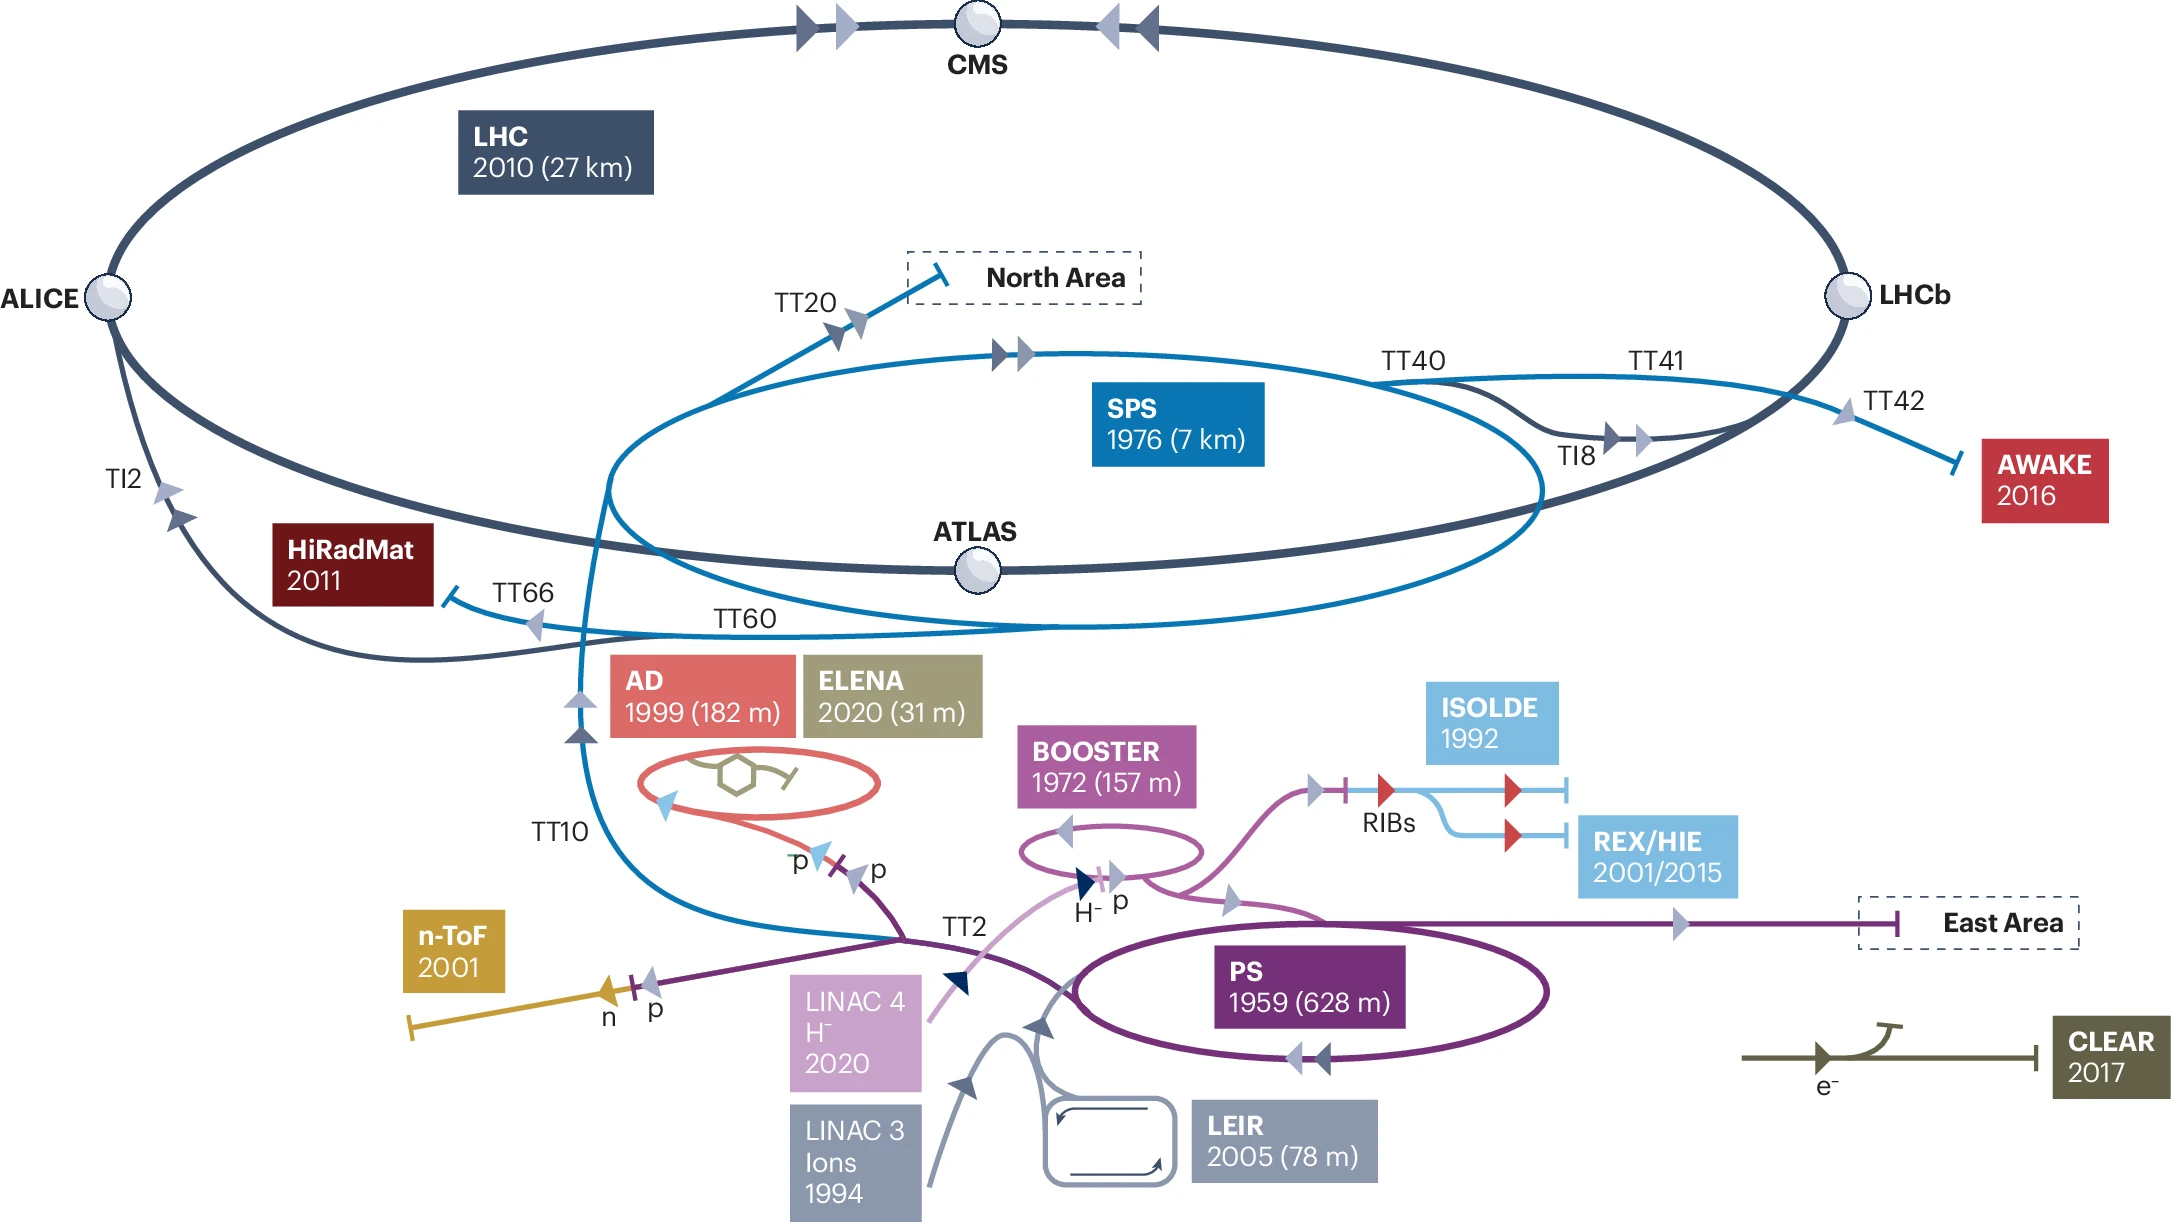
\includegraphics[width=1.0\textwidth]{images/CERN_Complex.png}
    \caption{Schematic overview of the CERN accelerator complex including main synchrotron accelerators LHC, SPS 
    and PS.}
    \label{fig:CERN_Complex}
\end{figure}

Achieving the desired collision energies requires the use of mutliple components of the CERN accelerator complex 
\ref{fig:CERN_Complex}, which consists of linear and smaller circular colliders that were operated as independent 
experiments in the past. The acceleration is facilitated by an intricate setup of magnets (mostly dipoles and quadrupoles), 
which also steer and focus the beams. For proton-proton collisions this process starts with $H^-$ ions which are 
accelerated to $160\ MeV$ by a linear accelerator called Linac4. From there the ions are injected into the circular  
Proton Synchrotron Booster (PSB), which strips both electrons from the Hydrogen ions and creates a pure proton beam with 
an energy of $2\ GeV$. Afterwards the beam is accelerated to $26\ GeV$ by the Proton Synchrotron (PS) and $450\ GeV$ by the Super Proton Synchrotron (SPS) before finally being injected into the LHC where it reaches its final collision energy. 
\par

%https://home.cern/news/news/accelerators/accelerator-report-excellent-2024-lhc-run-ended-abruptly
\begin{table}
\begin{center}
\caption{Overview of run periods of the LHC between 2008 and 2026.}
\label{table-lhc-runs}
\begin{tabular}{|c c c c|} 
 \hline
 Run Number & Years & Center of mass energy & Integrated Luminosity \\ [0.5ex] 
 \hline
 1 & 2008-2013 & $7-8\ TeV$ & $29.2\ fb^{-1}$ \\ 
 2 & 2015-2018 & $13\ TeV$ & $159.8\ fb^{-1}$ \\ 
 3 & 2022-2026 & $13.6\ TeV$ & $195.9\ fb^{-1}$ (up to and including 2024) \\ 
 \hline
\end{tabular}
\end{center}
\end{table}

The LHC has been operational since 2008, when it recorded its first proton-proton collisions at a center of mass energy 
of $7\ TeV$. Operation has been split into three distinct run periods denoted runs 1, 2 and 3 with shutdowns in 
between for maintenance and accelerator upgrades. Details on the timeline of these runs, alongside achieved energy and 
luminosity is shown in table \ref{table-lhc-runs}. Run 1 is mostly relevant for historical reasons and this thesis will 
focus on data collected during runs 2 and 3 given the much higher center of mass energy. The LHC presents the backdrop 
for the research of thousands of physicists spread across the ATLAS, CMS, ALICE and LHCb collaborations as well as 
multiple smaller teams at any given time. It is the best tool we have available to study the kinds of most fundamental 
particle interactions we are interested in.

\section{The ATLAS Detector}

ATLAS (\textbf{A} \textbf{T}oroidal \textbf{L}HC \textbf{A}pparatu\textbf{S}) is the largest of the four main detectors 
around the LHC ring. It is a general purpose detector designed to record the proton-proton collision signatures 
generated in LHC collisions without focusing too heavily on any specific processes, requiring trade-offs in detector 
design. It is around 46 meters long with a diameter of 25 meters and weights around 7000 tons. The detector 
\ref{fig:ATLAS_detector} consists of four main active components: an inner tracking detector, a calorimeter system and 
a muon spectrometer, which interact with different types of particles \ref{fig:Detector_Interactions}. The inner 
tracking detector is responsible for precise trajectory measurements of charged particles and represents the most 
intricate part of the ATLAS detector. The calorimeter system is used to measure the energy of electrons and photons 
(electromagnetic calorimeter) as well as hadrons (hadronic calorimeter). Finally the muon system identifies muons 
penetrating the rest of the detector. In order to make accurate measurements of particle momentum, the ATLAS detector 
uses a magnet system to curve the trajectories of charged particles. All of these elements will be discussed in more 
detail in this section.

%https://cerncourier.com/a/atlas-undergoes-some-delicate-gymnastics/
\begin{figure}
\centering
    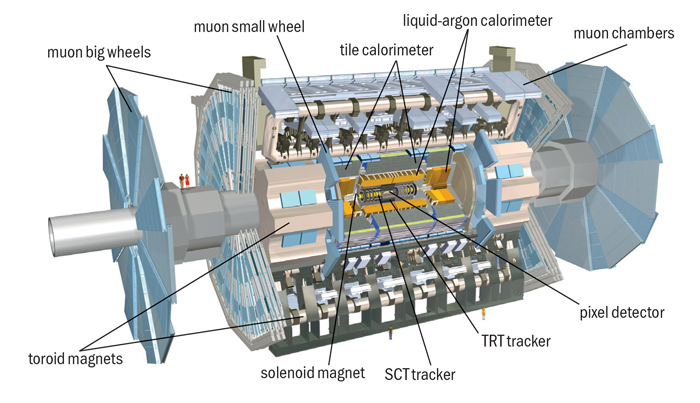
\includegraphics[width=1.0\textwidth]{images/ATLAS_Detector.jpg}
    \caption{Diagram showing all components of the ATLAS detector.}
    \label{fig:ATLAS_Detector}
\end{figure}

%https://www.nbi.dk/~petersen/Teaching/Stat2011/Project1/project1.html
\begin{figure}
\centering
    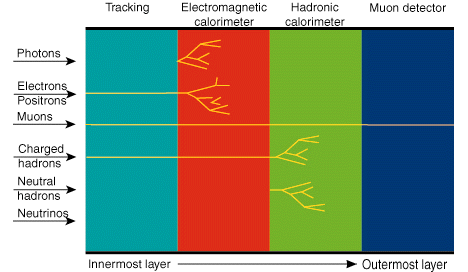
\includegraphics[width=1.0\textwidth]{images/Detector_Interactions.png}
    \caption{Sketch showing how different particles interact with detector components.}
    \label{fig:Detector_Interactions}
\end{figure}

\subsection{Inner tracking detector}

\section{Object Reconstruction}